\apendice{Especificación de diseño}

\section{Introducción}

En este anexo se recogen las características de diseño de \textit{software} que implementan los requisitos previamente explicados.

\section{Diseño de datos}

En ``Fastastic Roads'' no hay ningún tipo de base de datos o elementos que se le asemejen, pues se trata de un videojuego. De igual manera, cuenta con diferentes entidades, especialmente controladores, que conforman el buen funcionamiento del juego como uno de carreras contrarreloj.

Entre los principales controladores esenciales se encuentra el controlador de carrera. Con ``RaceController'' se ha mantenido una relación directa con los \textit{checkpoints} para el control de los mismos y su correcto funcionamiento en el circuito. Estos \textit{checkpoints} dependen entre sí para el debido transcurso de la carerra, permitiendo al vehículo bifurcaciones por distintos caminos donde pudiese haber puntos de control diferentes sin que esto afectara a la imposibilidad de finalizar una partida. 

\imagen{race-con-check}{Diagrama de clases de ``Race Controller'' y ``Checkpoint''.}

\section{Diseño procedimental}

La ejecución de la aplicación es sencilla, puesto que la aplicación se ejecuta bajo un único núcleo exportado desde Unity.

\begin{figure}[h]
	\centering
	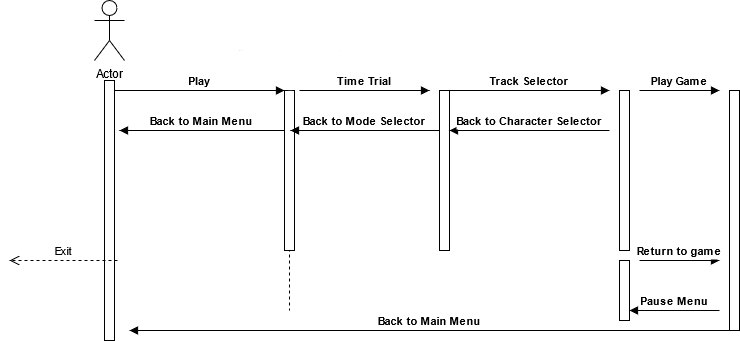
\includegraphics[width=\textwidth]{seq-diag}
	\caption{Diagrama de secuencias de ``Fastastic Roads''.}
	\label{fig:seq-diag}
\end{figure}

El usuario, con la aplicación ejecutada, selecciona las distintas opciones a través de los botones mostrados en pantalla que le llevarán a nuevos menús hasta acabar en una partida, pudiendo salir posteriormente de ella.

\section{Diseño arquitectónico}

En ``Fastastic Roads'' se han aplicado algunos patrones de diseño a la hora de desarrollar el proyecto. Unity permite la implementación de patrones estandarizados, como el ``Modelo-Vista-Controlador''. A continuación, se procede a explicar los patrones implementados.

\subsection{Patrón estrategia}

Mediante la implementación de este patrón de comportamiento, se permite al algoritmo variar independientemente de los clientes que lo utilizan. Aplicado al proyecto, el control en el videojuego se abstrae, materializándose en distintas estrategias (para el control local de un jugador o multijugador, control en red, etc.) para poder incluir nuevas funcionalidades sin tener que modificar el código independientemente de quién los utiliza \cite{disman:estrat}.

\imagen{patron-estrategia}{Estructura del patrón de comportamiento estrategia.}

\subsection{Patrón método fábrica}

El método fábrica es un patrón creacional que nos permite definir una interfaz para crear un objeto, pero son las subclases quienes deciden la clase a instanciar, i.e., se delega la instanciación a las subclases \cite{disman:metfab}. En el caso de ``Fastastic Roads'', hemos requerido de su uso en algunos métodos relacionados con el controlador de \textit{karts}.

\imagen{patron-metodo-fabrica}{Estructura del patrón creacional método fábrica}

\subsection{Patrón método plantilla}

En el patrón de comportamiento método plantilla se define el esqueleto de un algoritmo en una operación, dejando algunos de los pasos para las subclases, para que éstas redefinan ciertos pasos del algoritmo sin cambiar su estructura general \cite{disman:metplan}.

En este proyecto, por una parte se utilizan controles universales, donde cada uno tendrá una implementación específica que no interfiera con el resto de jugadores, y así se abstraen los controles a niveles altos.

\imagen{patron-metodo-plantilla}{Estructura del patrón creacional método plantilla.}

\section{Diseño de interfaces}

Por último, respecto al diseño de interfaz se decidió por elementos simples.

Un buen diseño en una aplicación donde los componentes gráficos son notables y muy importantes de cara a la buena recepción del usuario como son los videojuegos, es muy importante. Sin embargo, en el desarrollo de un videojuego la interfaz, así como otros tantos elementos y funcionalidades del mismo, no se perfecciona dejándolo visualmente llamativo hasta que la aplicación está bastante avanzada, e incluso cercana a terminar.

No obstante, eso no implica que se tenga que descuidar, pues ha de ser accesible al usuario tanto en el juego final como en las fases de desarrollo. Por ello, se decidió la colocación de botones grandes en los distintos menús, fáciles de entender y eficientes con su función asignada.

\imagen{fastastic-design-menu}{A pesar de la carencia de colores y un diseño atractivo, un usuario medio es capaz de entenderlo fácilmente.}

A medida que el proyecto vaya creciendo y se vayan creando nuevas funcionalidades, los menús tendrán tipografías más agradables a la vista y los botones serán más llamativos que los actualmente asignados.

Respecto al juego en sí, es importante tener una buena implementación de las distintas funciones para poder disfrutar de él, pero con un mal diseño puede acabar aburriendo o cansando al usuario. Es por ello que este aspecto es más importante tenerlo trabajado desde un principio, por lo que el juego tiene escenarios altamente detallados y llamativos, así como unos diseños de vehículos que invitan al usuario a disfrutar de una conducción divertida con ellos.

\imagen{fastastic-design-track}{Los escenarios se han trabajado desde un principio, permitiendo mejoras a medida que se avanza con el proyecto.}

A ello se le añade un buen diseño de logotipo para la identificación del videojuego. Este logotipo tuvo una fase previa, y ahora mismo es el diseño final disponible con el cual se puede distinguir a ``Fastastic Roads''.

\imagen{fastastic-roads-logo}{El logotipo de ``Fastastic Roads'' apela a la estética industrial del videojuego.}